\documentclass[12pt,letterpaper]{article}

\usepackage{pdfpages}
\usepackage{hyperref}
\usepackage[title, titletoc, toc]{appendix}
\usepackage{graphicx}
\usepackage{xspace}

\begin{document}

% definitions here

\title{SSim Roadmap for DC1 Production}
\author{ .. (add names/affiliations) ...$^1$, C.W.~Walter$^2$ \\
{\small $^1$SLAC National Accelerator Laboratory, $^2$Duke University}}

\date{\today}

\maketitle

\begin{abstract}
  In this note we describe and document the configurations used for
  the DESC DC1 data challenge including the validation metrics for
  certification of suitability for the science studies described in
  the 2015 DESC Science Roadmap document~\cite{SRM:2015}.
\end{abstract}

\noindent
\begin{center}
  \fboxsep=5pt \fbox{\begin{minipage}{5.25in} \it This document is in
      initial draft form.  Add your name and expand the text.  Authors
      should include SSim, LSS, Clusters and CI members.
    \end{minipage}} 
  \end{center} 
\vspace{0.1in}

\section{Introduction}

At the March 2016 SLAC collaboration meeting the SSim group surveyed
and discussed with the analysis working groups their needs for DC1
production. This was a followup to the original proposal as laid out
in the SRM~\cite{SRM:2015} after the analysis groups had further time
to determine their needs.  After the meeting, C. Walter followed up
with the groups determining both which ones would use the common DC1
data sets and coming to a common set of initial specifications for the
production to be carried about by the Computer Infrastructure (CI)
group.

This document summarizes the consensus list of the needed parameters
and configuration options and serves as a record of the options used
in the production.  Additionally, in this document we specify the
tests used to validate that an initial test sample of produced images
are appropriate.

\section{Groups Using the DC1 Simulation}

For DC1 simulation not all groups will be using the PhoSim based
output.  The following group {\bf will not use} the DC1 based
output:

\begin{enumerate}
\item The Weak Lensing (WL) group is using GalSim for this round
  of tests. 
\item The Strong Lensing (SL) and Supernova (SN) groups are using
  Twinkles\cite{Twinkles:2016}, a PhoSim based deep field oversampled
  with lenses and supernovae.  The Twinkles production is also serving
  as a path-finding effort by allowing the CI group to build the
  infrastructure needed to produce, track and process large numbers of
  image planes.  We plan to utilize the same system for the DC1
  production.
\end{enumerate}

The following groups {\bf will use} the DC1 based output and are the
main contributors and users of this document:

\begin{enumerate}
\item The Large Scale Structure (LSS) group will use the PhoSim based
  output to start to test their algorithms and strategies.
\item The Clusters (Cl) group will mostly use the output of DC1 to
  inform their needs for the DC2 simulation round.
\end{enumerate}

After discussion between the LSS and Cl groups a common set of initial
configurations was agreed to. Summaries of the group needs are found
in a spreadsheet located in Appendix~\ref{sec:survey}.

\section{DC1 Configuration Options}

The options chosen for the DC1 production are for the most part a
further specification or refinement on the specifications of the 'DC1
PhoSim Deep data set as described in Table 4.1.1 in the
SRM~\cite{SRM:2015}. The summary spreadsheet in
Appendix~\ref{sec:survey} collates the options given by the working
group with some refinement after discussion with C. Walter.  In that
table, yellow boxes represent consensus choices and orange boxes are
requests for specialized followup  data sets. It should be noted that
in some cases the choice of tool necessitates the configuration.  For
example, in PhoSim vignetting is an emergent phenomena and cannot be
turned off.

Table~\ref{tab:phosim-options} describes the choice of options for
production as extracted from the survey results.

\begin{table}[!htb]
  \centering
  \begin{tabular}{| l| l| }
    \hline 
    Parameter                       & Value   \\
    \hline
    Catalog and Image area  & 80 sq deg \\
    Number of Visits            & 150 visits per pointing \\
    Bands                             & r   \\
    Cadence                         & OpSim WFD  \\
    Input                              & {\bf Tentative} Standard CatSim catalog \\
    Sky Model                      & Basic OpSim Model \\
    Dithering                       & Random translational and rotational  \\
    Clouds                           & {\bf Tentative} yes \\
    Sensor Effects                & Only saturation and blooming \\
    \hline
  \end{tabular}
  \caption{Catalog and PhoSim Options}
  \label{tab:phosim-options}
\end{table}

Additionally, the LSS group has asked for {\bf specialized follow-up
  runs} with 1) All sensor effects turned on and 2) added dithering
pattern(s).  Production of these will be samples will be evaluated
after the initial DC1 data set has been evaluated by the LSS group.

The PhoSim command file which implement the cloud and sensor effects (but not the
instance catalog files) can be found in Appendix~\ref{sec:command-file}.  The
CatSim query commands can be found in~ ??? {\bf (Can we document this?)}.

\section{Output Format and Processing}

Both the LSS and Clusters group expect FITS files to be produced and
tracked.  The Clusters group seems to only need image files.  \\

\noindent
{\bf DOES LSS OR CLUSTERS NEED DM PROCESSING BY CI?} \\
 
\noindent
Exactly what is needed here needs to be fleshed out.

\section{Validation Samples and Tests}

Before running the full production we plan to make some smaller test
runs to ensure that things are being done properly and the output
(including any processing) is usable by the LSS and Clusters group. \\


\noindent
{\bf SPECIFY SAMPLES AND VALIDATION TESTS HERE}


\section{Timeline}

The entries in this document should be agreed to by the LSS, Clusters,
SSim and CI groups during the Oxford meeting.  Test production should
begin soon after that with the schedule being set by the CI group.

\begin{appendices}

\section{Survey Responses}
\label{sec:survey}

A PDF export of a summary of the survey responses is found here.  Both
the PDF and (full) xls file can be found in the same repository as the
source of this document:
\url{https://github.com/DarkEnergyScienceCollaboration/SSim_DC1_Roadmap}.

In this table a blank entry means that the responders did not care,
Yellow boxes constitute commonly agreed parameters among the groups.
Orange boxes represent requested follow up data sets for the LSS group.

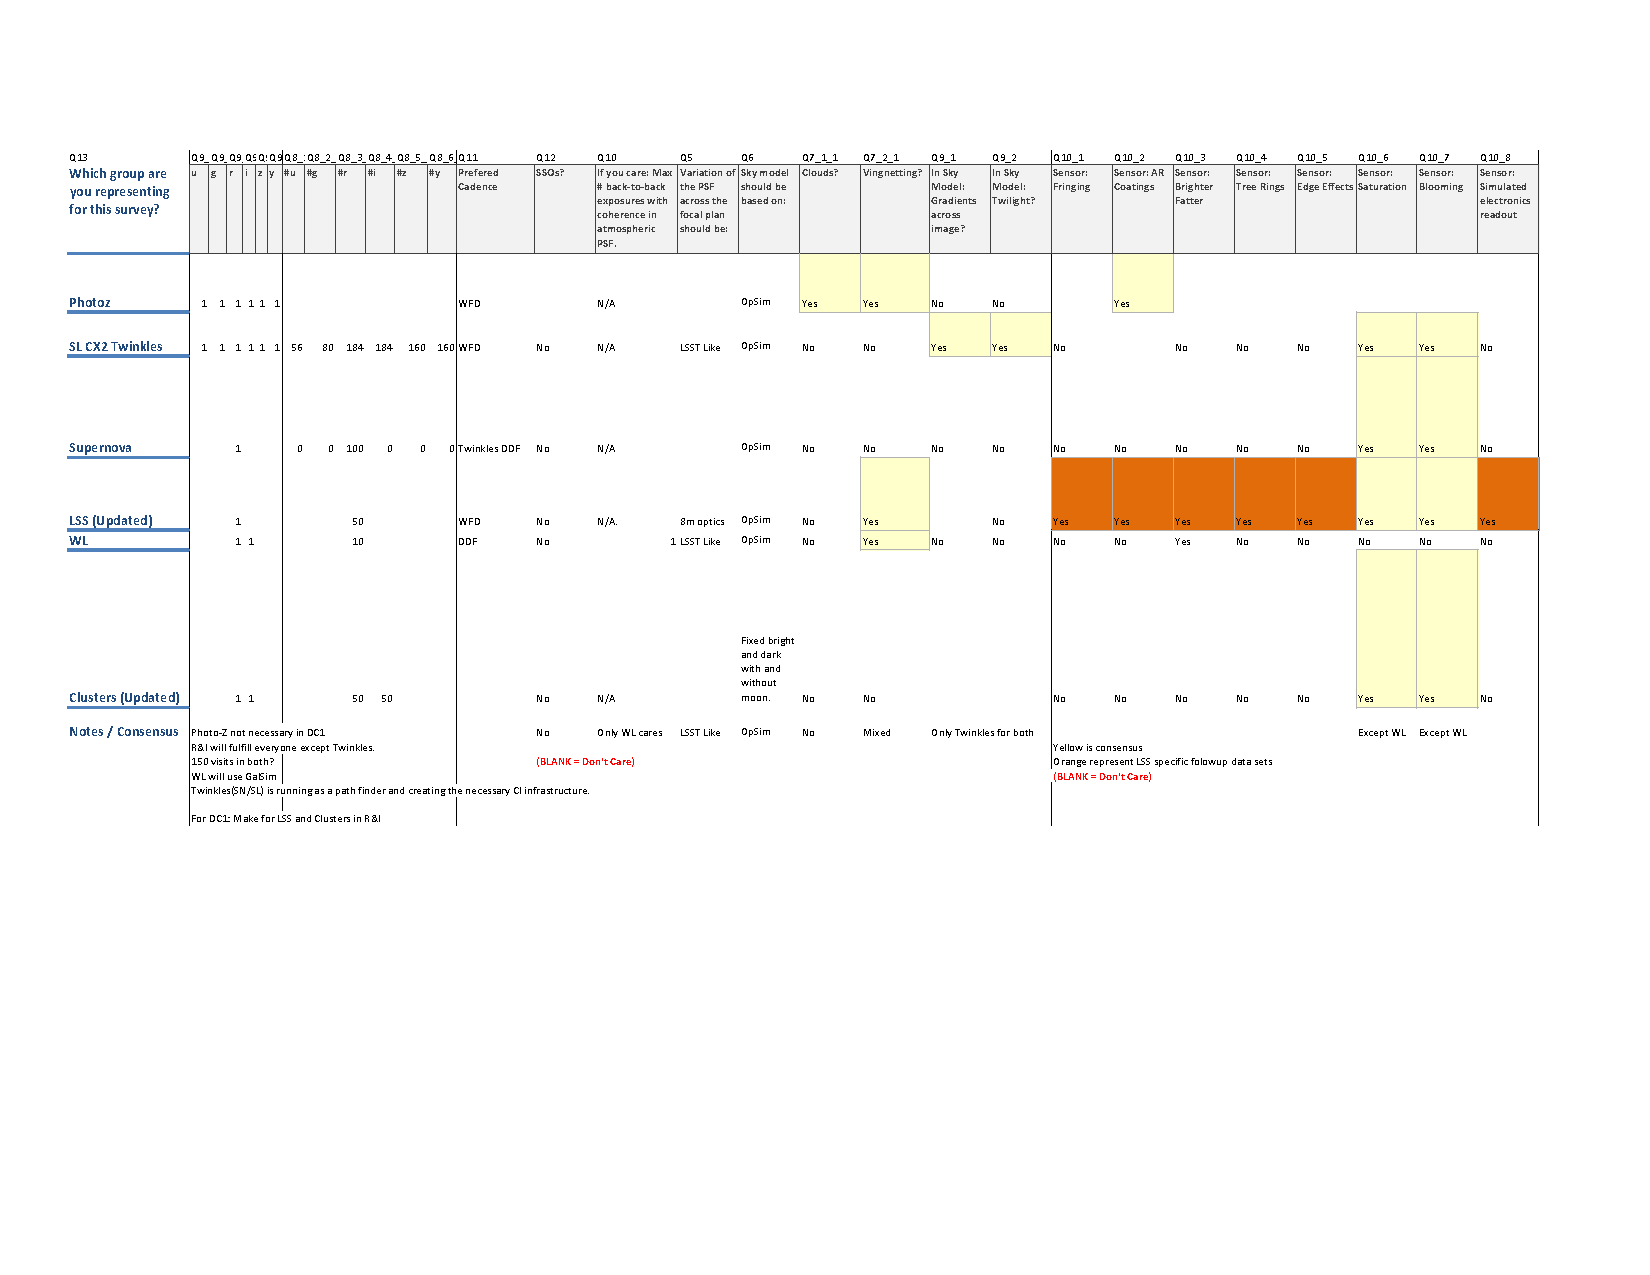
\includepdf[pages=1,angle=90]{Simulation_Requirements_Survey.pdf} 

\section{PhoSim Command File}
\label{sec:command-file}

The basic PhoSim command file used to run the production should be
included here.

\begin{verbatim}
Lots O\' Commands
\end{verbatim}

\end{appendices}

\begin{thebibliography}{100}

\bibitem{SRM:2015} 
DESC Science Roadmap,
\url{http://lsst-desc.org/sites/default/files/DESC_SRM_V1.pdf}, 2015

\bibitem{Twinkles:2016} Twinkles,
  \url{https://github.com/DarkEnergyScienceCollaboration/Twinkles},
  2016

\end{thebibliography}

\end{document}
